\documentclass[12pt]{article}
\usepackage[margin=1.5cm]{geometry}
\usepackage{tikz}
\usetikzlibrary{arrows.meta,bending,positioning}
\pagestyle{empty}

\tikzset{
  st/.style={circle, draw=black, fill=white,
             minimum size=7mm, font=\scriptsize, inner sep=0pt},
  tr/.style={-{Stealth[scale=0.55]}, very thin, black},
  sl/.style={-{Stealth[scale=0.4]}, very thin, black,
             min distance=5mm, looseness=6},
  init/.style={-{Stealth[scale=0.55]}, very thin, black},
}

\begin{document}

% ====================================================
%  HYP 1
% ====================================================
\begin{center}
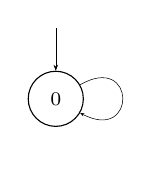
\begin{tikzpicture}
  \node[st] (s0) at (0,0) {0};
  \draw[init] (0,0.9) -- (s0);
  \path (s0) edge[sl, out=30, in=330] (s0);
\end{tikzpicture}
\end{center}

\clearpage

% ====================================================
%  HYP 2  --  vertical column: 0 -> 1 -> 2
% ====================================================
\begin{center}
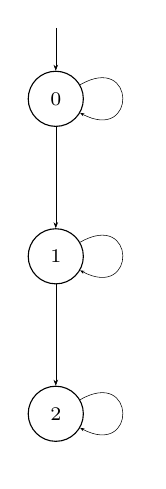
\begin{tikzpicture}
  \node[st] (s0) at (0,0)    {0};
  \node[st] (s1) at (0,-2)   {1};
  \node[st] (s2) at (0,-4)   {2};

  \draw[init] (0,0.9) -- (s0);

  \path (s0) edge[sl, out=30, in=330] (s0);
  \path (s1) edge[sl, out=30, in=330] (s1);
  \path (s2) edge[sl, out=30, in=330] (s2);

  \path (s0) edge[tr] (s1);
  \path (s1) edge[tr] (s2);
\end{tikzpicture}
\end{center}

\clearpage

% ====================================================
%  HYP 3  --  0 at top, 1+3 in middle, 2 at bottom
% ====================================================
\begin{center}
\begin{tikzpicture}
  \node[st] (s0) at (0,0)     {0};
  \node[st] (s1) at (1.2,-2)  {1};
  \node[st] (s3) at (-1.2,-2) {3};
  \node[st] (s2) at (1.2,-4)  {2};

  \draw[init] (0,0.9) -- (s0);

  \path (s0) edge[sl, out=30,  in=330] (s0);
  \path (s1) edge[sl, out=30,  in=330] (s1);
  \path (s2) edge[sl, out=30,  in=330] (s2);
  \path (s3) edge[sl, out=150, in=210] (s3);

  \path (s0) edge[tr] (s1);
  \path (s0) edge[tr] (s3);
  \path (s1) edge[tr] (s2);
  \path (s3) edge[tr, bend left=10] (s1);
\end{tikzpicture}
\end{center}

\clearpage

% ====================================================
%  HYP 4  --  adds s4 below s2
% ====================================================
\begin{center}
\begin{tikzpicture}
  \node[st] (s0) at (0,0)     {0};
  \node[st] (s1) at (1.2,-2)  {1};
  \node[st] (s3) at (-1.2,-2) {3};
  \node[st] (s2) at (1.2,-4)  {2};
  \node[st] (s4) at (1.2,-6)  {4};

  \draw[init] (0,0.9) -- (s0);

  \path (s0) edge[sl, out=30,  in=330] (s0);
  \path (s1) edge[sl, out=30,  in=330] (s1);
  \path (s2) edge[sl, out=30,  in=330] (s2);
  \path (s3) edge[sl, out=150, in=210] (s3);
  \path (s4) edge[sl, out=30,  in=330] (s4);

  \path (s0) edge[tr] (s1);
  \path (s0) edge[tr] (s3);
  \path (s1) edge[tr] (s2);
  \path (s2) edge[tr] (s4);
  \path (s3) edge[tr, bend left=10] (s1);
\end{tikzpicture}
\end{center}

\clearpage

% ====================================================
%  HYP 5  --  adds s5 between s1 and s4
% ====================================================
\begin{center}
\begin{tikzpicture}
  \node[st] (s0) at (0,0)     {0};
  \node[st] (s1) at (1.2,-2)  {1};
  \node[st] (s3) at (-1.2,-2) {3};
  \node[st] (s2) at (2.2,-4)  {2};
  \node[st] (s5) at (0.2,-4)  {5};
  \node[st] (s4) at (1.2,-6)  {4};

  \draw[init] (0,0.9) -- (s0);

  \path (s0) edge[sl, out=30,  in=330] (s0);
  \path (s1) edge[sl, out=30,  in=330] (s1);
  \path (s2) edge[sl, out=30,  in=330] (s2);
  \path (s3) edge[sl, out=150, in=210] (s3);
  \path (s5) edge[sl, out=150, in=210] (s5);
  \path (s4) edge[sl, out=30,  in=330] (s4);

  \path (s0) edge[tr] (s1);
  \path (s0) edge[tr] (s3);
  \path (s1) edge[tr] (s2);
  \path (s1) edge[tr] (s5);
  \path (s2) edge[tr] (s4);
  \path (s3) edge[tr, bend left=10] (s1);
  \path (s5) edge[tr] (s4);
\end{tikzpicture}
\end{center}

\clearpage

% ====================================================
%  HYP 6  --  adds s6 below s3
% ====================================================
\begin{center}
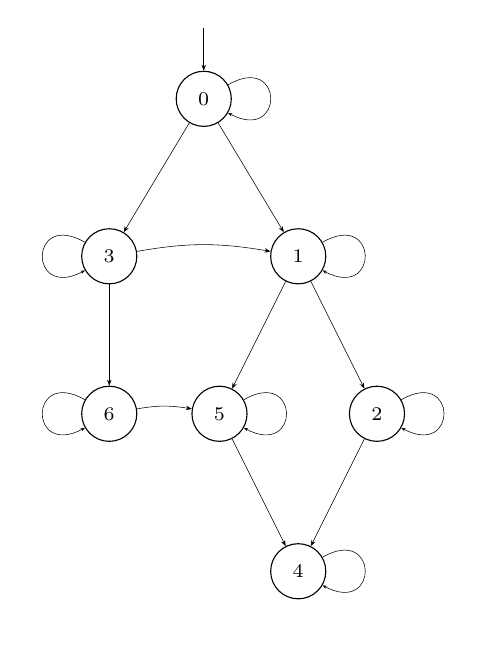
\begin{tikzpicture}
  \node[st] (s0) at (0,0)      {0};
  \node[st] (s1) at (1.2,-2)   {1};
  \node[st] (s3) at (-1.2,-2)  {3};
  \node[st] (s2) at (2.2,-4)   {2};
  \node[st] (s5) at (0.2,-4)   {5};
  \node[st] (s6) at (-1.2,-4)  {6};
  \node[st] (s4) at (1.2,-6)   {4};

  \draw[init] (0,0.9) -- (s0);

  \path (s0) edge[sl, out=30,  in=330] (s0);
  \path (s1) edge[sl, out=30,  in=330] (s1);
  \path (s2) edge[sl, out=30,  in=330] (s2);
  \path (s3) edge[sl, out=150, in=210] (s3);
  \path (s5) edge[sl, out=30,  in=330] (s5);
  \path (s6) edge[sl, out=150, in=210] (s6);
  \path (s4) edge[sl, out=30,  in=330] (s4);

  \path (s0) edge[tr] (s1);
  \path (s0) edge[tr] (s3);
  \path (s1) edge[tr] (s2);
  \path (s1) edge[tr] (s5);
  \path (s2) edge[tr] (s4);
  \path (s3) edge[tr, bend left=10]  (s1);
  \path (s3) edge[tr] (s6);
  \path (s5) edge[tr] (s4);
  \path (s6) edge[tr, bend left=10]  (s5);
\end{tikzpicture}
\end{center}

\end{document}
